\subsection{Project Organization}
\progname{}'s development uses the general software development life cycle
processes of requirements analysis, architecture and design definition,
implementation, verification, and validation. Each of these processes outputs at
least one Software Development Artifact (SDA) which serves as a description of
the process's results and becomes an input to subsequent processes
(Figure~\ref{fig:dependencies}). Each SDA has an associated verification and/or
validation plan (Table~\ref{tab:verificationPlanLocation}) to ensure that it
adheres to the \progname{}'s concept.

\vspace*{\fill}
\begin{figure}[!h]
    \centering
    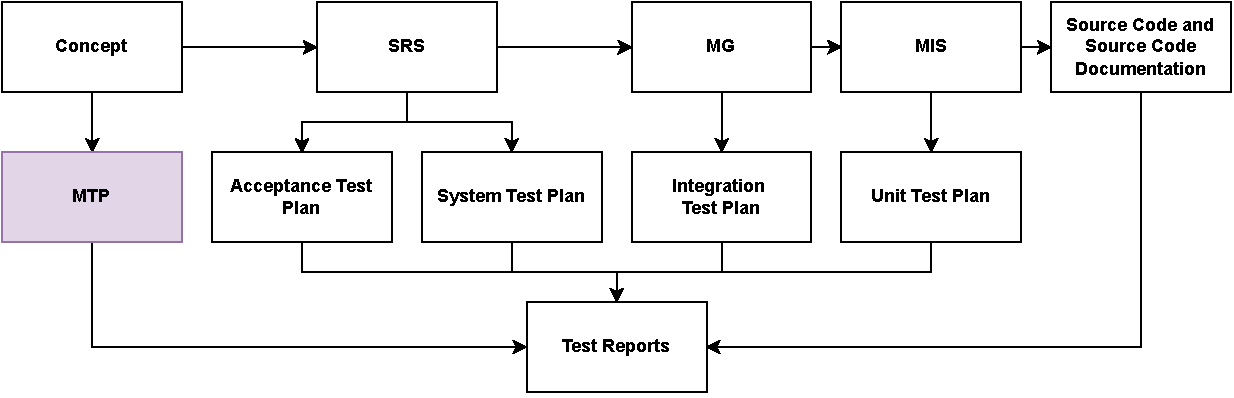
\includegraphics[width=\textwidth]{figures/mtpOrg.pdf}
    \caption{Dependencies Between \progname{}'s SDAs (MTP Highlighted)}
    \label{fig:dependencies}
\end{figure}

\begin{table}[!h]
    \renewcommand{\arraystretch}{1.2}
    \centering
    \caption{Location of V \& V Plans for \progname{}'s SDAs}
    \label{tab:verificationPlanLocation}
    \begin{tabular}{P{0.38\linewidth}P{0.5\linewidth}}
        \toprule
        \textbf{SDA} & \textbf{Location of V \& V Plan} \\

        \midrule

        \colourRow Concept Summary & -- \\

        Master Test Plan & Master Test Plan \\

        \colourRow Software Requirements Specification & Master Test Plan \\

        Module Guide & Master Test Plan \\

        \colourRow Module Interface Specification & Master Test Plan \\

        System, Integration, and Unit Test Plan & Master Test Plan \\

        \colourRow Acceptance Test Plan & Master Test Plan \\

        Source Code and Source Code Documentation& System, Integration, and
        Unit Test Plan \newline Acceptance Test Plan \\

        \bottomrule
    \end{tabular}
\end{table}
\vspace*{\fill}